%! TeX root = /Users/trustinnguyen/Downloads/Berkeley/Math/Math143/Homework/Math143Hw8/Math143Hw8.tex

\documentclass{article}
\usepackage{/Users/trustinnguyen/.mystyle/math/packages/mypackages}
\usepackage{/Users/trustinnguyen/.mystyle/math/commands/mycommands}
\usepackage{/Users/trustinnguyen/.mystyle/math/environments/article}
\graphicspath{{./figures/}}

\title{Math143Hw8}
\author{Trustin Nguyen}

\begin{document}

    \maketitle

\reversemarginpar

\textbf{Exercise 1}: Check the following statements from class:
    \begin{itemize}
        \item [(a)] If $\varphi :X \rightarrow Y$ is an isomorphism that sends $P$ to $Q$, then $\varphi^{*}: \mathcal{O}_{Q}(Y) \rightarrow \mathcal{O}_{P}(X)$ is an isomorphism.
            \begin{proof}
                Since $\varphi$ is an isomorphism, we find that there is a $\psi$ such that $\psi\varphi = id$. So we have 
                    \begin{equation*}
                        \psi\varphi(P) = \psi(Q) = P
                    \end{equation*}
                Furthermore, we can say there exists a $\psi^{*} : \Gamma(X) \rightarrow \Gamma(Y)$ such that $\psi^{*}\varphi^{*} = id$ and $\varphi^{*}\psi^{*} = id$. Then proved in lecture was that $\varphi^{*}: \mathcal{O}_{Q}(Y) \rightarrow \mathcal{O}_{P}(X)$ is well defined if we have the mapping:
                    \begin{equation*}
                        \varphi^{*}(\dfrac{g}{h}) = \dfrac{\varphi^{*}(g)}{\varphi^{*}(h)}
                    \end{equation*}
                and also,
                    \begin{equation*}
                        \varphi^{*}(h)(P) = h(\varphi(P)) = h(Q) \neq 0
                    \end{equation*}
                Now if we define $\psi^{*}$ as:
                    \begin{equation*}
                        \psi^{*}(\dfrac{g}{h}) = \dfrac{\psi^{*}(g)}{\psi^{*}(h)}
                    \end{equation*}
                for $g$, $h$ in $\Gamma(X)$ and $\frac{g}{h} \in \mathcal{O}_{P}(X)$. Then using the fact that $\psi(Q) = P$, we get:
                    \begin{equation*}
                        \psi^{*}(h)(Q) = h(\psi(Q)) = h(P) \neq 0
                    \end{equation*}
                This tells us that $\frac{\psi^{*}(g)}{\psi^{*}(h)} \in \mathcal{O}_{Q}(Y)$ and the denominator is not the zero polynomial. Now we see that:
                    \begin{equation*}
                        \varphi^{*}\psi^{*}(\dfrac{g}{h}) = \dfrac{\varphi^{*}\psi^{*}(g)}{\varphi^{*}\psi^{*}(h)} = \dfrac{g}{h}
                    \end{equation*}
                since $\varphi^{*}\psi^{*} = id_{\Gamma(X)}$. Now because $\psi^{*}\varphi^{*} = id_{\Gamma(Y)}$, we have:
                    \begin{equation*}
                        \psi^{*}\varphi^{*}(\dfrac{g}{h}) = \dfrac{\psi^{*}\varphi^{*}(g)}{\psi^{*}\varphi^{*}(h)} = \dfrac{g}{h}
                    \end{equation*}
                So both compositions are identities. So $\varphi^{*}$ is an isomorphism.
            \end{proof}

        \item [(b)] Let $P = (0, 0)$. Prove directly from the definition that $I_{P}(x, y) = 1$.
            \begin{proof}
                By definition, we have:
                    \begin{equation*}
                        I_{P}(x, y) = \dim_{k}\left(\dfrac{\mathcal{O}_{P}(\mathbb{A}^{2})}{(x, y)}\right)
                    \end{equation*}
                Let $f(x, y), g(x, y)$ have non-zero constant term. We will show that $\frac{k_{1}}{f(x, y)}$ is a generator of $\mathcal{O}_{P}(\mathbb{A}^{2})/(x, y)$. Suppose that $\frac{k_{2}}{g(x, y)} \in \mathcal{O}_{P}(\mathbb{A}^{2})/(x, y)$. Then observe that we desire a $k_{0} \in k$ such that:
                    \begin{equation*}
                        \left(\dfrac{k_{1}}{f(x, y)}\right) \cdot k_{0} = \dfrac{k_{2}}{g(x, y)}
                    \end{equation*}
                we get:
                    \begin{align*}
                        k_{1}k_{0}g(x, y) &= k_{2}f(x, y)                   \\
                        k_{1}k_{0}g_{0}   &= k_{2}f_{0} \mod{(x, y)}                    \\
                        k_{0}             &= k_{2}f_{0}k_{1}^{-1}g_{0}^{-1} \in k  
                    \end{align*}
                So we have found a $k_{0}$. Then $\frac{k_{1}}{f(x, y)}$ is a generator of $\mathcal{O}_{P}(\mathbb{A}^{2})/(x, y)$. So it is one-dimensional.
            \end{proof}

        \item [(c)] Suppose $f$ and $g$ have no repeated factors, $P$ is a smooth point of $V(f)$ and $V(g)$ and the tangent lines to $V(f)$ and $V(g)$ at $P$ are distinct. Prove that $I_{P}(f, g) = 1$. 
            \begin{proof}
                If $P \neq 0$, then first compute the pullback and everything will be preserved, such as the multiplicity of $P$ in $f, g$, the distinct tangent lines, and that $P$ is smooth. Because the tangent lines are distinct, we know that $I_{P}(f, g) = \mult_{P}(f)\mult_{P}(g)$. Because $P$ is smooth, by the formula for a tangent line:
                    \begin{align*}
                        f_{x}(p)(x - x_{0}) + f_{y}(p)(y - y_{0}) &= 0 \\
                        g_{x}(p)(x - x_{0}) + g_{y}(p)(y - y_{0}) &= 0   
                    \end{align*}
                we know that there is exactly one tangent line for $f$, called $T_{f}$, and one for $g$, called $T_{g}$. So $V(T_{f}), V(T_{g})$ are the tangent cones of $f, g$. And we see that both $T_{f}, T_{g}$ are homogeneous of degree $1$, therefore, $\mult_{P}(f) = 1$ and $\mult_{P}(g) = 1$. So the product is equal to $I_{P}(f, g) = 1$.
            \end{proof}
    \end{itemize}

\textbf{Exercise 2}: Let $P = (0, 0)$ and $k = \mathbb{C}$. Compute the following intersection numbers using the properties from class. There may be many possible routes to do so!
    \begin{itemize}
        \item [(a)] $I_{P}(x^{2} - y, y^{2} - x^{3})$
            \begin{answer}
                We have
                    \begin{align*}
                        I_{P}(x^{2} - y, y^{2} - x^{3}) &= I_{P}(y^{2} - y, x^{2} - y)                   \\
                                                        &= I_{P}(y, x^{2} - y) + I_{P}(y - 1, x^{2} - y) \\
                                                        &= I_{P}(y, x^{2})                               \\
                                                        &= 2I_{P}(x, y)                                  \\
                                                        &= 2                                               
                    \end{align*}
            \end{answer}

        \item [(b)] $I_{P}(x - y^{2}, x + y^{2})$
            \begin{answer}
                We have
                \begin{align*}
                    I_{P}(x - y^{2}, x + y^{2}) &= I_{P}(2x, x + y^{2}) \\
                                                &= I_{P}(x, x + y^{2})  \\
                                                &= I_{P}(x, y^{2})      \\
                                                &= 2I_{P}(x, y)         \\
                                                &= 2                      
                \end{align*}
            \end{answer}

        \item [(c)] $I_{P}(x^{3} + xy, 3x^{2}y + xy^{2})$
            \begin{answer}
                We have
                    \begin{align*}
                        I_{P}(x^{3} + xy, 3x^{2}y + xy^{2}) &= I_{P}(xy, x^{3} + xy) + I_{P}(x^{3} + xy, 3x + y) \\
                                                            &= I_{P}(xy, x^{3}) + I_{P}(x^{3} - 3x^{2}, 3x + y)  \\
                                                            &= I_{P}(x, x^{2}) + I_{P}(x^{3} - 3x^{2}, 3x + y)   \\
                                                            &= \infty                                              
                    \end{align*}
            \end{answer}

        \item [(d)] $I_{P}(x + y + y^{2}x, x + y + x^{2} - y^{2} + y^{3})$ 
            \begin{answer}
                We have
                    \begin{align*}
                        I_{P}(x + y + y^{2}x, x + y + x^{2} -y^{2} + y^{3}) &= I_{P}(x^{2} - y^{2} + y^{3} - y^{2}x, x + y + y^{2}x)                                          \\
                                                                            &= I_{P}(y^{2}(y - x) + (-1)(x - y)(x + y), x + y + y^{2}x)                                       \\
                                                                            &= I_{P}((y^{2} - 1)(y - x)(x + y), x + y + y^{2}x)                                               \\
                                                                            &= I_{P}(y^{2} - 1, x + y + y^{2}x) + I_{P}(y - x, x + y + y^{2}x) + I_{P}(x + y, x + y + y^{2}x) \\
                                                                            &= 0 + I_{P}(y - x, x + y + y^{2}x) + I_{P}(x + y, x + y + y^{2}x)                                \\
                                                                            &= I_{P}(y - x, 2y + y^{2}x) + I_{P}(x + y, y^{2}x)                                               \\
                                                                            &= I_{P}(y, y - x) + I_{P}(y - x, 2 + yx) + I_{P}(x + y, y^{3})                                   \\
                                                                            &= I_{P}(y, x) + 0 + 3I_{P}(x + y, y)                                                             \\
                                                                            &= I_{P}(x, y) + 3I_{P}(x, y)                                                                     \\
                                                                            &= 4I_{P}(x, y)                                                                                   \\
                                                                            &= 4                                                                                                
                    \end{align*}
            \end{answer}
    \end{itemize}

\textbf{Exercise 3}: Let $g, h \in k[x, y]$ and let $P = (0, 0)$.
    \begin{itemize}
        \item [(a)] Prove that $I_{P}(y, g + h) \geq \min(\{I_{P}(y, g), I_{P}(y, h)\})$
            \begin{proof}
                If $g(x, 0) = 0$, then $y \divides g$ and so we can say that $I_{P}(y, g + h) = I_{P}(y, h)$ because $g \in(y)$. The vanishing of $g$ and $y$ have a common component so $I_{P}(y, g) = \infty$, and therefore, $I_{P}(y, h) \geq I_{P}(y, h)$ which is true. If both $g(x, 0) = 0 = h(x, 0)$, then the above equation turns to:
                    \begin{equation*}
                        I_{P}(y) \geq \min(I_{P}(y), I_{P}(y))
                    \end{equation*}
                which is true. So suppose that $y  \ndivides g, h$. Then we can write $I_{P}(y, g) = I_{P}(y, g^{\prime})$ and the same for $h \rightarrow h^{\prime}$ for $g^{\prime}, h^{\prime}$ polynomials in terms of $x$. And then $(y, g + h) = (y, g^{\prime} + h^{\prime})$. So we have:
                    \begin{align*}
                        g^{\prime}(x) &= g_{0} + g_{1} + \cdots \\
                        h^{\prime}(x) &= h_{0} + h_{1} + \cdots   
                    \end{align*}
                Let $g_{i}$ be the first non-zero homogeneous form in $g^{\prime}$ and $h_{k}$ be the first non-zero homogeneous form in $h^{\prime}$. Then we have:
                    \begin{align*}
                        g^{\prime} &= x^{i}(g_{0} + g_{1} + \cdots) \\
                        h^{\prime} &= x^{k}(h_{0} + h_{1} + \cdots)   
                    \end{align*}
                by factoring out the $x^{\prime}s$ and note that $g_{0}, h_{0} \neq 0$. Then
                    \begin{align*}
                        I_{P}(y, g^{\prime}) &= I_{P}(x^{i},y) + I_{P}(g_{0} + g_{1} + \cdots, y) & I_{P}(y, h^{\prime}) &= I_{P}(x^{k}, y) +kI_{P}(h_{0} + h_{1} + \cdots, y) \\
                                             &= i + 0                                             &   &= k + 0                                                
                    \end{align*}
                We note that $I_{P}(g_{0} + g_{1} + \cdots, y) = 0$ because the $y$ vanishes on $(0, 0)$ but the $g_{0} + g_{1} + \cdots$ does not because $g_{0} \neq 0$. So the RHS turns out to be
                    \begin{equation*}
                        \min(i, k)
                    \end{equation*}
                While
                    \begin{equation*}
                        I_{P}(y, g + h) = I_{P}(y, g^{\prime} + h^{\prime})
                    \end{equation*}
                and we note that $g^{\prime} + h^{\prime}$ has multiplicity greater than or equal to $g^{\prime}$ and $h^{\prime}$. So in the same process above,
                    \begin{equation*}
                        g^{\prime} + h^{\prime} = (g^{\prime} + h^{\prime})_{0} + (g^{\prime} + h^{\prime})_{1} + \cdots
                    \end{equation*}
                and the first non zero homogeneous form is at least $\min(i, k)$. So repeating the process gives us $I_{P}(y, g + h) \geq \min(i, k)$, so we are done.
            \end{proof}

        \item [(b)] It turns out part $(a)$ is true whenever we replace $y$ with a polynomial $f$ such that $f_{1} \neq 0$ (but you do not need to prove this). However, it can be false when $f_{1} = 0$. Find an example of polynomials $f, g$ and $h$ so that $I_{P}(f, g + h) <  \min(\{I_{P}(f, g), I_{P}(f, h)\})$. 
            \begin{proof}
                The counterexample is at the end if explanation isn't needed.

                To construct an example, we see that:
                    \begin{align*}
                        I_{P}(f, g + h) &\geq \mult_{P}(f)\mult_{P}(g + h) \\
                                        &\geq \mult_{P}(f)\min(\mult_{P}(g), \mult_{P}(h)) \\
                                        &= \min(\mult_{P}(f)\mult_{P}(g), \mult_{P}(f)\mult_{P}(h))
                    \end{align*}
                So we want $I_{P}(f, g) \neq \mult_{P}(f)\mult_{P}(g)$ and $I_{P}(f, h) \neq \mult_{P}(f)\mult_{P}(h)$. Otherwise, we get $I_{P}(f, g + h) \geq \min(I_{P}(f, g), I_{P}(f, h))$. So this means that the $f, g$ share some tangent line and $f, h$ share some tangent line. But we want $g + h$ to not share a tangent line with $f$ to minimize $I_{P}(f,g + h)$. Considering:
                    \begin{center}
                        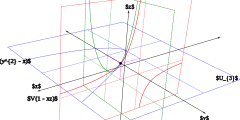
\includegraphics[scale=.8]{Exercise3}
                    \end{center}
                We see that $g = x + y$, $h = x - y$ satisfy the requirements and $g + h = 2x$ has no tangent lines in common with $x^{2} - y^{2}$. So to verify:
                    \begin{align*}
                        I_{P}(f, g) &= I_{P}(x^{2} - y^{2}, x + y) & I_{P}(f, h) &= I_{P}(x^{2} - y^{2}, x - y) & I_{P}(f, g + h) &= I_{P}(x^{2} - y^{2}, 2x)          \\
                                    &= \infty                      &             &= \infty                      &                 &= I_{P}(x - y, x) + I_{P}(x + y, x) \\
                                    &                              &             &                              &                 &= 1 + 1 = 2                           
                    \end{align*}
                And indeed, $I_{P}(f, g + h) < \infty$. Let $P = (0, 0)$. We have:
                    \begin{equation*}
                        I_{P}(x^{2} - y^{2}, 2x) < \min(I_{P}(x^{2} - y^{2}, x - y), I_{P}(x^{2} - y^{2}, x + y))
                    \end{equation*}
            \end{proof}
    \end{itemize}

\textbf{Exercise 4}: Nodes: Let $f \in k[x, y]$ be a polynomial with no repeated factors. We say that $f$ has a node at $P$ if $P$ has multiplicity $2$ in $V(f)$ and the tangent cone of $f$ is two distinct lines. Prove that $P$ is a node of $V(f)$ if and only if $f_{xy}(P) \neq f_{xx}(P)f_{yy}(P)$. Here $f_{xy} = \dv{x}(\dv{y}f)$ and $f_{xx} = \dv[2]{x}f$ and $f_{yy} = \dv[2]{y}f$ are second derivatives.
    \begin{proof}
        Suppose that $P$ has multiplicity $2$ in $V(f)$. Then it also has multiplicity $2$ in the pullback where if $P = (p_{1}, p_{2})$:
            \begin{equation*}
                \varphi(x, y) = (x + p_{1}, y + p_{2})
            \end{equation*}
        and
            \begin{equation*}
                \varphi^{*}f(x, y) = f(x + p_{1}, y + p_{2})
            \end{equation*}
        So we will consider $\varphi^{*}f$ and $(0, 0) \in V(\varphi^{*}f)$. Since we know that it has multiplicity $2$ also, we have that $V(\varphi^{*}f_{2})$ is the tangent cone, which decomposes into $V(L_{1}L_{2})$ where $L_{1}, L_{2}$ are distinct lines. Then
            \begin{align*}
                L_{1} &: y = a_{1}x \\
                L_{2} &: y = a_{2}x   
            \end{align*}
        And
            \begin{equation*}
                L_{1}L_{2} = (y - a_{1}x)(y - a_{2}x) = y^{2} - (a_{1} + a_{2})xy  + a_{1}a_{2}x^{2}
            \end{equation*}
        Notice that since
            \begin{equation*}
                f = f_{2} + f_{3} + \cdots+f_{m}
            \end{equation*}
        Then $f_{xy}(P), f_{xx}(P), f_{yy}(P)$ are determined only by $(f_{2})_{xx}(P), (f_{2})_{yy}(P), (f_{2})_{xy}(P)$, as the homogeneous terms of higher degree will still contain a $x$ or $y$ variable and evaluate to $0$ upon plugging in $P = (0, 0)$. Then:
            \begin{align*}
                (f_{2})_{xx} &= 2a_{1}a_{2}      \\
                (f_{2})_{xy} &= -(a_{1} + a_{2}) \\
                (f_{2})_{yy} &= 2                  
            \end{align*}
        Then
            \begin{equation*}
                f_{xy}^{2}(P) = a_{1}^{2} + 2a_{1}a_{2} + a_{2}^{2} = 4a_{1}a_{2} = f_{xx}(P)f_{yy}(P)
            \end{equation*}
        implies that
            \begin{equation*}
                a_{1}^{2} - 2a_{1}a_{2} + a_{2}^{2} = 0
            \end{equation*}
        which means that $(a_{1} - a_{2})^{2} = 0$ or $a_{1} = a_{2}$ which is a contradiction. So $f_{xy}^{2}(P) \neq f_{xx}(P)f_{yy}(P)$. This argument also works in reverse because we made no non-arbitrary assumptions about $f_{2}$. So its iff.
    \end{proof}

\textbf{Exercise 5}: Cusps: Let $f \in k[x, y]$ be a polynomial with no repeated factors and suppose $P$ is a point of multiplicity $2$ in $V(f)$. Furthermore, suppose now that the tangent cone of $V(f)$ is a single line $V(L)$.
    \begin{itemize}
        \item [(a)] Show that $I_{P}(f, L) \geq 3$. If equality holds, we say $V(f)$ has a cusp at $P$.
            \begin{proof}
                We know that intersection multiplicity is preserved with a change of coordinates, so we can look at $I_{(0, 0)}(\varphi^{*}f, \varphi^{*}L)$ where $\varphi^{*}$ is some translation. By the fact that:
                    \begin{equation*}
                        I_{P}(f, g) \geq \mult_{P}(f)\mult_{P}(g)
                    \end{equation*}
                we have
                    \begin{equation*}
                        I_{(0, 0)}(\varphi^{*}f, \varphi^{*}L) \geq \mult_{(0, 0)}(\varphi^{*}f)\mult_{(0, 0)}(\varphi^{*}L) = 2 \cdot
                    \end{equation*}
                But because $(0, 0)$ as a point in $f$ has multiplicity $2$ with tangent line $L$ in common, equality does not hold, so in fact,
                    \begin{equation*}
                        I_{(0, 0)}(\varphi^{*}f, \varphi^{*}L) \geq3
                    \end{equation*}
                the translation is an isomorphism, and is invertible, so we know that $I_{P}(f, L) \geq3$.
            \end{proof}

        \item [(b)] Suppose $P = (0, 0)$ and $L = y$. Show that $P$ is a cusp if and only if $f_{xxx}(P) \neq 0$, where $f_{xxx}$ is the third partial derivative of $f$ with respect to $x$.
            \begin{proof}
                 We have that
                    \begin{equation*}
                        f = f_{2} + f_{3} + \cdots
                    \end{equation*}
                Since $P = (0, 0)$, with multiplicity $2$, we know that $V(f_{2}) = V(y)$, as the tangent cone. Then $V(f_{2}) = V(A) \cup V(B) = V(y)$, but $V(y)$ is irreducible, so we know that $A = y, B = y$, as neither of the vanishings can be empty. Now looking at the $f_{3}$ term, 
                    \begin{equation*}
                        f_{3} = a_{3}x^{3} + a_{2}x^{2}y + a_{1}xy^{2} + y^{3}
                    \end{equation*}
                Calculating $(f_{3})_{xxx}(P)$, we get:
                    \begin{equation*}
                        (f_{3})_{xxx}(P) = 6a_{3}
                    \end{equation*}
                In the context of $f$, we have:
                    \begin{equation*}
                        f_{xxx}(P) = (f_{2})_{xxx}(P) + (f_{3})_{xxx}(P) + (f_{4})_{xxx}(P) + \cdots
                    \end{equation*}
                And because all terms of $(f_{i})_{xxx}$ for $i >3$ contain either an $x$ or a $y$, we know that evaluation at $P$ returns $0$, so:
                    \begin{equation*}
                        f_{xxx}(P) = (f_{3})_{xxx}(P) = 6a_{3}
                    \end{equation*}
                Suppose that $f_{xxx}(P) \neq 0$. We will prove a cusp, with a chain of iffs. Then
                    \begin{equation*}
                        f_{xxx}(P) \neq 0 \iff 6a_{3} \neq 0 \iff a_{3} \neq 0
                    \end{equation*}
                Then $a_{3}x^{3}$ is a summand of $f$ and $y \ndivides f$. We know that
                    \begin{equation*}
                        I_{P}(f, L) = I_{P}(y^{2} + f_{3} + \cdots, y) = I_{P}(f_{3} + \cdots, y)
                    \end{equation*}
                reducing the right polynomial $f_{3} + f_{4} + \cdots$ into a polynomial in terms of just $x$, we get:
                    \begin{align*}
                        I_{P}(f, L) &= I_{P}(a_{3}x^{3} + a_{4}x^{4} + \cdots + a_{n}x^{n}, y) \\
                                    &= I_{P}(a_{3} + a_{4}x + \cdots + a_{n}x^{n - 3}, y) + I_{P}(x^{3}, y) \\
                                    &= 3I_{P}(x, y) + I_{P}(a_{3} + a_{4}x + \cdots + a_{n}x^{n - 3}, y) \\
                                    &= 3 + I_{P}(a_{3} + a_{4}x + \cdots + a_{n}x^{n - 3}, y)
                    \end{align*}
                But we know that $a_{3} \neq 0$. So $(0, 0) \notin V(a_{3} + a_{4}x + \cdots + a_{n}x^{n - 3})$. This means that the intersection multiplicity for the right summand is $0$. So we have
                    \begin{equation*}
                        I_{P}(f, L) = 3
                    \end{equation*}
                The chain of iffs means that this is a biconditional.
            \end{proof}

        \item [(c)] Show that if $P$ is a cusp, then $V(f)$ has only one irreducible component passing through $P$. 
            \begin{proof}
                If $P$ is a cusp at $V(f)$, then we can do some change of coordinates by translation or rotations to get that $(0, 0)$ has the same multiplicity as $P$ and that it is in $V(f^{\prime})$ where the tangent line at $P$ is $V(y)$. If $V(f) = V(g) \cup V(h)$ where both algebraic sets are proper subsets of $V(f)$, then suppose that they both contain $P$. We must have:
                    \begin{equation*}
                        I_{P}(f, g) = I_{P}(g, y) + I_{P}(h, y)
                    \end{equation*}
                We have three possibilities:
                    \begin{itemize}
                        \item The tangent cone of $V(g)$ is $y^{i}$ for $i \geq2$ (Sharing common tangent line with $y$). Then:
                            \begin{equation*}
                                I_{P}(g, y) = I_{P}(x^{k} + x^{k + 1} + \cdots)
                            \end{equation*}
                        where $k \geq3$. And we know that there is at least one $x^{i}$ term because $y \ndivides g$. Then $I_{P}(g, y) \geq3$, which is a contradiction because $I_{P}(h, y) \geq1$ and the total $I_{P} = 3$

                        \item The tangent cone of $V(g)$ shares no common factor with $y$. Then $I_{P}(g, y) = \mult_{P}(g)\mult_{P}(y) = \mult_{P}(g)$. Then $I_{P}(f, y) = \mult_{P}(g)  + \mult_{P}(h)$. Wlog, assume $\mult_{P}(g) = 1$. Then $g = k_{0}x + \cdots$ and $h = k_{2}x^{2} + k_{3}xy + k_{4}y^{2} + \cdots$. But this is a contradiction because $V(g) \cup V(h) = V(gh) = V(f)$. And $gh$ and $f$ now have different tangent cones, where the tangent cone of $gh$ is $a_{3}x^{3} + a_{2}x^{2}y + a_{1}xy^{2} + a_{0}y^{3}$ where $a_{3} \neq 0$. So it does not contain a $V(y)$ line.

                        \item If the tangent cone of $V(g), V(h)$ share at least one common factor, then we know that $I_{P}(g, y) = (x^{2} + \cdots)$ because the tangent cone is divisible by $y$ and terms that contain only $x$ are those that are homogeneous of degree at least $2$. Then $I_{P}(g, y) + I_{P}(h, y) \geq4 \neq 3$. So contradiction.
                    \end{itemize}
                So there is only one irreducible component passing through $P$.
            \end{proof}
    \end{itemize}

Optional: You may wish to look back at Homework $5$ problems $1$ and $2$. One had a node and one had a cusp - do you see which is which and prove it?

\begin{answer}
    The cusp is $(0, 0)$ in $V(x^{3} - y^{2})$ because $f_{xxx}((0, 0)) = 6 \neq 0$. This one is:
        \begin{center}
            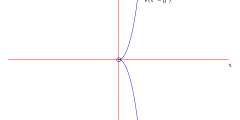
\includegraphics{cusp}
        \end{center}

    The node is $(0, 0)$ in $V(y^{2} - x^{3} + x^{2})$ because $f_{xx}(P) = 2$, $f_{yy}(P) = 2$, and $f_{xy}(P) = 0$. We have $f_{xy}^{2}(P) = 0 \neq 4 = f_{xx}(P)f_{yy}(P)$. This one is:
        \begin{center}
            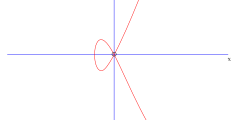
\includegraphics{node}
        \end{center}
\end{answer}

































\end{document}
